\documentclass[journal,twoside,web]{ieeecolor}
\usepackage{tmi}
\usepackage{cite}
\usepackage{amsmath,amssymb,amsfonts}
\usepackage{algorithmic}
\usepackage{graphicx}
\usepackage{textcomp}
\usepackage{lipsum} 
\usepackage{booktabs}
\usepackage[acronym]{glossaries}

\newacronym{CT}{CT}{computed tomography}
\newacronym{MRI}{MRI}{magnetic resonance imaging}
\newacronym{AI}{AI}{artificial intelligence }
\newacronym{LLMs}{LLMs}{large language models}
\newacronym{NSCLC}{NSCLC}{non-small cell lung cancer}

\newacronym[]{DCM}{DCM}{\textit{dilated cardiomyopathy}}
\newacronym[]{HCM}{HCM}{\textit{hypertrophic cardiomyopathy}}
\newacronym[]{NOR}{NOR}{\textit{normal}}
\newacronym[]{MINF}{MINF}{\textit{myocardial infarction}}
\newacronym[]{RV}{RV}{\textit{right Ventricular abnormality}}

\newacronym[]{SE}{SE}{\textit{squeeze and excitation}}

\def\BibTeX{{\rm B\kern-.05em{\sc i\kern-.025em b}\kern-.08em
    T\kern-.1667em\lower.7ex\hbox{E}\kern-.125emX}}
    
\markboth{\journalname, VOL. XX, NO. XX, XXXX 2025}
{Author \MakeLowercase{\textit{et al.}}: PreparationXXX of Papers for IEEE TRANSACTIONS ON MEDICAL IMAGING}

\begin{document}

\title{Magnetic Resonance Imaging Analysis for Cardiomyopathy Classification with Attention Mechanisms Support}

\author{
   Santiago. Diogo, \IEEEmembership{Fellow, IEEE},
   \thanks{Submitted to review at 27th February 2025.}


\thanks{Diogo Santiago and Leila Cristina C. Bergamasco are in the Electrical Engineering Postgraduate Program from University College FEI, São Bernardo do Campo, São Paulo State, Brazil. (e-mail: diogo.felipe.santiago@gmail.com; leila.cristina@fei.edu.br).}


}

\maketitle

% ---------------------------------------------
\begin{abstract}
The increasing availability of medical imaging exams, such as magnetic resonance imaging, generates a large volume of data, making its analysis complex and challenging. In this scenario, advanced computational approaches can optimize the interpretation of these images and assist in the early diagnosis of cardiovascular diseases. This work aims to unify contemporary approaches in the evaluation of cardiomyopathy. 
With the support of radiomic analysis, which extracts information from statistical and texture characteristics of a medical image, and features derived from a classical neural network for computer vision, such as ResNet50, promising results can combined and obtained \cite{heDeepResidualLearning2015}. Some forms of attention mechanism are applied including self attention and selective attention using Squeeze and Excitation Nets.  The results confirm that the combination of information from various domains regarding a given patient, when integrated, can lead to more interesting outcomes compared to analyzing data in isolation. This study aims to apply the aforementioned approaches, based on previous literature, in an innovative application for cardiomyopathy testing.
% , adapting and proposing a more robust architecture 
% to achieve better results.
\end{abstract}

% ---------------------------------------------
\begin{IEEEkeywords}
Radiomics, Attention Mechanism, Transformers, Cardiomyopathy, Medical Imaging.
\end{IEEEkeywords}

% ---------------------------------------------
\section{Introduction}
\label{sec:introduction}
\IEEEPARstart{S}{ince} the early 2000s, the volume of data generated in medicine has grown exponentially,this rapid growth highlights the need for tools capable of efficiently processing and analyzing vast amounts of information.

Medical imaging techniques, such as \gls{CT} and \gls{MRI}, have become essential in modern medicine, offering detailed three-dimensional representations of human anatomy. These imaging techniques not only improve diagnostic accuracy but also generate large datasets that can be quantitatively analyzed. Concurrently, \gls{AI} has driven significant advancements in diagnostic imaging, enhancing efficiency and precision in medical decision-making.

Deep neural networks have demonstrated high performance in computer vision tasks, including image classification, object detection, and segmentation. Once optimized on a given dataset, these models can extract discriminative features that enhance medical image analysis. Furthermore, transformer architectures, commonly used in autoregressive generative models such as \gls{LLMs}, have gained prominence due to their parallelization capabilities and self-attention mechanisms, which allow models to focus on the most relevant parts of the input data.

Additionally, image processing techniques such as texture analysis have been employed for decades in various medical domains. Radiomics, a powerful approach for extracting quantitative features from medical images, captures patterns that may not be perceptible to the human eye. This methodology has shown potential applications in fields such as oncology and cardiology \cite{mayerhoeferIntroductionRadiomics2020}.

In cardiac imaging analysis, texture-based MRI assessments have been used to evaluate the risk of post-myocardial infarction arrhythmia. Specifically, texture analysis of contrast-enhanced and non-contrast MRI scans in cardiomyopathy patients has been explored for predicting clinical outcomes \cite{schofieldTextureAnalysisCardiovascular2019a}. Among cardiomyopathies, \gls{HCM} is one of the most prevalent, frequently diagnosed in young and middle-aged individuals. While often asymptomatic, \gls{HCM} can lead to severe conditions such as heart failure and stroke, making early diagnosis crucial in preventing adverse outcomes. In this context, radiomics—which extracts high-dimensional data from medical images, often including texture analysis—holds promise for early diagnosis and risk assessment in cardiomyopathy \cite{kwonComparisonMortalityCause2022}.

The integration of AI and radiomics represents a promising strategy for detecting cardiomyopathies and other cardiac conditions. Recent studies have demonstrated that combining deep features with radiomic characteristics can significantly improve the predictive performance of diagnostic models for lung cancer using CT imaging. Models leveraging self-attention mechanisms to analyze concatenated data have achieved up to 82.35\% accuracy and an AUC of 0.74 \cite{lambinRadiomicsExtractingMore2012}.

Thus, this study proposes the implementation and validation of a fusion strategy that combines radiomic and deep learning features with self-attention mechanisms to improve cardiomyopathy classification. Beyond advancing the state-of-the-art in medical diagnosis, this research aims to contribute to the development of more effective and accessible solutions for clinical decision support \cite{brielerCardiomyopathyOverview2017}.


% \IEEEPARstart{T}{his} document is a template for \LaTeX.
% You are encouraged to use it to prepare your manuscript.
% If you are reading a paper or PDF version of this document, please download the 
% \LaTeX .zip file from the IEEE Web site at \underline
% {https://www.embs.org/tmi/authors-instructions/} to prepare your manuscript.
% You can also explore using the Overleaf editor at 
% \underline
% {https://www.overleaf.com/blog/278-how-to-use-overleaf-with-}\discretionary{}{}{}\underline
% {ieee-collabratec-your-quick-guide-to-getting-started\#.}\discretionary{}{}{}\underline{xsVp6tpPkrKM9}

% ---------------------------------------------
\section{Dataset}
Two datasets were used in this study: ACDC and SunnyBrook. Both are publicly available and intended for research purposes. The ACDC dataset consists of 150 images, with 100 for training and 50 for testing, evenly distributed across five classes: DCM, HCM, NOR, MINF, and RV. The SunnyBrook dataset contains 45 images, and to maintain proportional compatibility with ACDC, it was divided into 30 images for training and 15 for testing. The dataset includes the following classes: NOR, IC, IC-I, and HIP. Details about each class are provided in the following sections dedicated to each dataset.

% ------
\subsection{ACDC Dataset}
The ACDC dataset was created using real clinical exams obtained from the University Hospital of Dijon (France). The acquired data was fully anonymized and processed in compliance with the regulations established by the local ethics committee of the Dijon hospital.  

This dataset covers several well-defined pathologies, with a sufficient number of cases to: (1) properly train machine learning methods, and  
(2) clearly evaluate variations in key physiological parameters derived from cine-MRI, particularly diastolic volume and ejection fraction.  

The dataset consists of $150$ exams, $100$ for training and $50$ for test. Each exam is from a different patient and the dataset is divided into five equally distributed subgroups. The five distinct classes are: \gls{DCM}, \gls{HCM}, \gls{NOR}, \gls{MINF}, and \gls{RV}. The \gls{DCM} and \gls{HCM} classes are interpreted as indicative of cardiomyopathy, while \gls{NOR}, \gls{MINF}, and \gls{RV} represent normal heart conditions. Details on these classes can be found in Table \ref{table01}.  

Additionally, the dataset includes segmentation masks, allowing for potential segmentation applications. The label values range from 0 to 3, representing voxels associated with the background (0), right ventricle cavity (1), myocardium (2), and left ventricle cavity (3). Figures 17, 18, and 19 illustrate the images and their respective segmentation masks for \gls{DCM}, \gls{HCM}, and NOR. These masks display three distinct shades of gray corresponding to the described segmentation.


\begin{table}[h]
\centering
\caption{ACDC Labels}
\label{table01}
\setlength{\tabcolsep}{4pt}
% \begin{tabular}{|p{32pt}|p{33pt}|p{72pt}|p{72pt}|}
\begin{tabular}{|c|c|c|c|}
    \hline 
          \textbf{Group} & \textbf{Quantity} & \textbf{W/ Cardiomiopaty} & \textbf{W/O Cardiomiopaty}  \\ 
    \hline 
        NOR & 30 & 0 & 30 \\ 
        DCM & 30 & 30 & 0\\ 
        HCM & 30 & 30 & 0\\ 
        MINF & 30 & 0 & 30 \\ 
        RV & 30 & 0 & 30 \\
    \hline 
        \textbf{Total}: & 150  & 60 & 90\\ 
    \hline 
    \multicolumn{4}{p{230pt}}{ACDC - Redistribution for normal $\times$ cardiomyopathy classification. } \\
\end{tabular} 
\end{table}


% ------
\subsection{SunnyBrook Dataset}
The Sunny dataset, also known as the 2009 Cardiac MR Left Ventricle Segmentation Challenge data, consists of 45 MRI images from a mixed group of patients and pathologies, including healthy individuals, hypertrophy, heart failure with infarction, and heart failure without infarction. There are four pathological groups in this dataset, classified as follows:  

a) Heart failure with infarction (IC-I): Group with an ejection fraction (EF) < 40\% and evidence of late gadolinium enhancement (Gd).  
b) Heart failure without infarction (IC): Group with EF < 40\% and no late gadolinium enhancement.  
c) Left ventricular hypertrophy (HIP): Group with normal EF ($>$ 55\%) and a left ventricular mass-to-body surface area ratio $>$ 83 g/m².  
d) Normal (NOR): Group with EF $>$ 55\% and no hypertrophy.  

For this study, the HIP and NOR classes were used to classify cases of cardiomyopathy and normal conditions, respectively. Table 6 shows the distribution of the 45 patients and the cardiovascular activity values used for patient classification .

% ---------------------------------------------
\section{Methodology}

In this section, first introduce the image preprocessing and feature extraction process, which involves selecting and extracting features from \gls{MRI} images. Then, we introduce the base model, originally applied to \gls{NSCLC} early recurrence prediction. And last, we describe the design of our proposed architecture with a new concatenation, using segmented masks and in addition to using the self-attention mechanism, it was also used selective attention in the form of \gls{SE} Net modules. 

Studies by \cite{huSqueezeandExcitationNetworks2018} demonstrated that network performance could be enhanced by explicitly incorporating learning mechanisms that help capture spatial correlations without requiring additional supervision.  In this context, the \gls{SE} mechanism was proposed to allow the network to recalibrate features, enabling it to learn how to use global information to selectively emphasize informative features while suppressing less useful ones \cite{lecunHandwrittenDigitRecognition1989}.

The change in the concatenation method was intentional, as the adapted version includes a new convolutional layer that is not present in the original version, aiming to extract relevant information from the fusion of embeddings. The adapted version also adds a selective attention layer in the form of an \gls{SE} block, which precedes the self-attention block \cite{osheaIntroductionConvolutionalNeural2015c}.  

Another modification in the adapted version is that the self-attention block is applied $N$ times instead of just once, as in the base work, leading to a noticeable improvement in results. It is important to note that both attention mechanisms serve different purposes: while the selective attention block focuses on the relationships between the embedding channels, the self-attention block efficiently optimizes and weights the fused feature vector.  

The intuition behind applying attention mechanisms with different purposes is inspired by the work of \cite{yangNeuralNetworkDesign2024a}.


% ------
\subsection{Data Preprocessing}

For the preprocessing step, the ACDC dataset was used. The ACDC dataset originally contains five distinct classes and we organized it for a binary cadyomiopathy classification. The set of frames used are defined in the diastolic phase, and the number of frames varies per patient. The radiomic features are extracted using the PyRadiomics library. This tool allows 3D cardiac image volumes and their respective masks to be used as input, extracting manual features related to texture, shape, grayscale intensity, etc.. The result is a vector of $78$ radiomic features.

Deep features are extracted using a ResNet50 network, excluding the final classification layer. This process is applied to each slice of the 3D volume for both the cardiac image and its corresponding mask, resulting in feature vectors of size $100,352$. Following the base model's methodology, an F-Test is applied to reduce the dimensionality from: deep features from 100,352 to 27,372 and radiomic features from 78 to $\text{EMBED}_{size} \in \{24, 48, 64\}$.

The $\text{EMBED}_{size}$ value varies in the adapted versions, serving as a hyperparameter, ensuring that all embeddings have the same size. Feature concatenation is performed: In the last dimension for the original model and its variations and in the first dimension for adapted versions. It is important to note that, unlike the base model version, which contains only one deep feature vector, the adapted versions may include an additional vector corresponding to the mask with the region of interest.

% ------
\subsection{Base Model}

The work from Ai et al (2023) proposed a deep learning based on self-attention mechanism for \gls{NSCLC} early recurrence prediction. Firstly radiomics was applied using diverse machine learning techniques to extract handcrafted features from \gls{CT} images, encompassing texture, shape, grayscale, etc. Radiomics-based methods mainly rely on handcrafted design to extract numerous quantitative  features from \gls{CT} images, including tumor shape, size, density,  texture, edge, etc \cite{aiSelfAttentionBasedFusion2023}

Subsequently, a pre-trained ResNet50 network was utilized to extract deep features that encapsulate high-level semantic and representation information from the \gls{CT} images. These features were then fused into a unified feature vector and a self attention module was applied ending with a classification layer for the \gls{NSCLC} early recurrence prediction \cite{aiSelfAttentionBasedFusion2023}. The architecture can be seen in Figure \ref{fig01}.


\begin{figure}[h]
\centerline{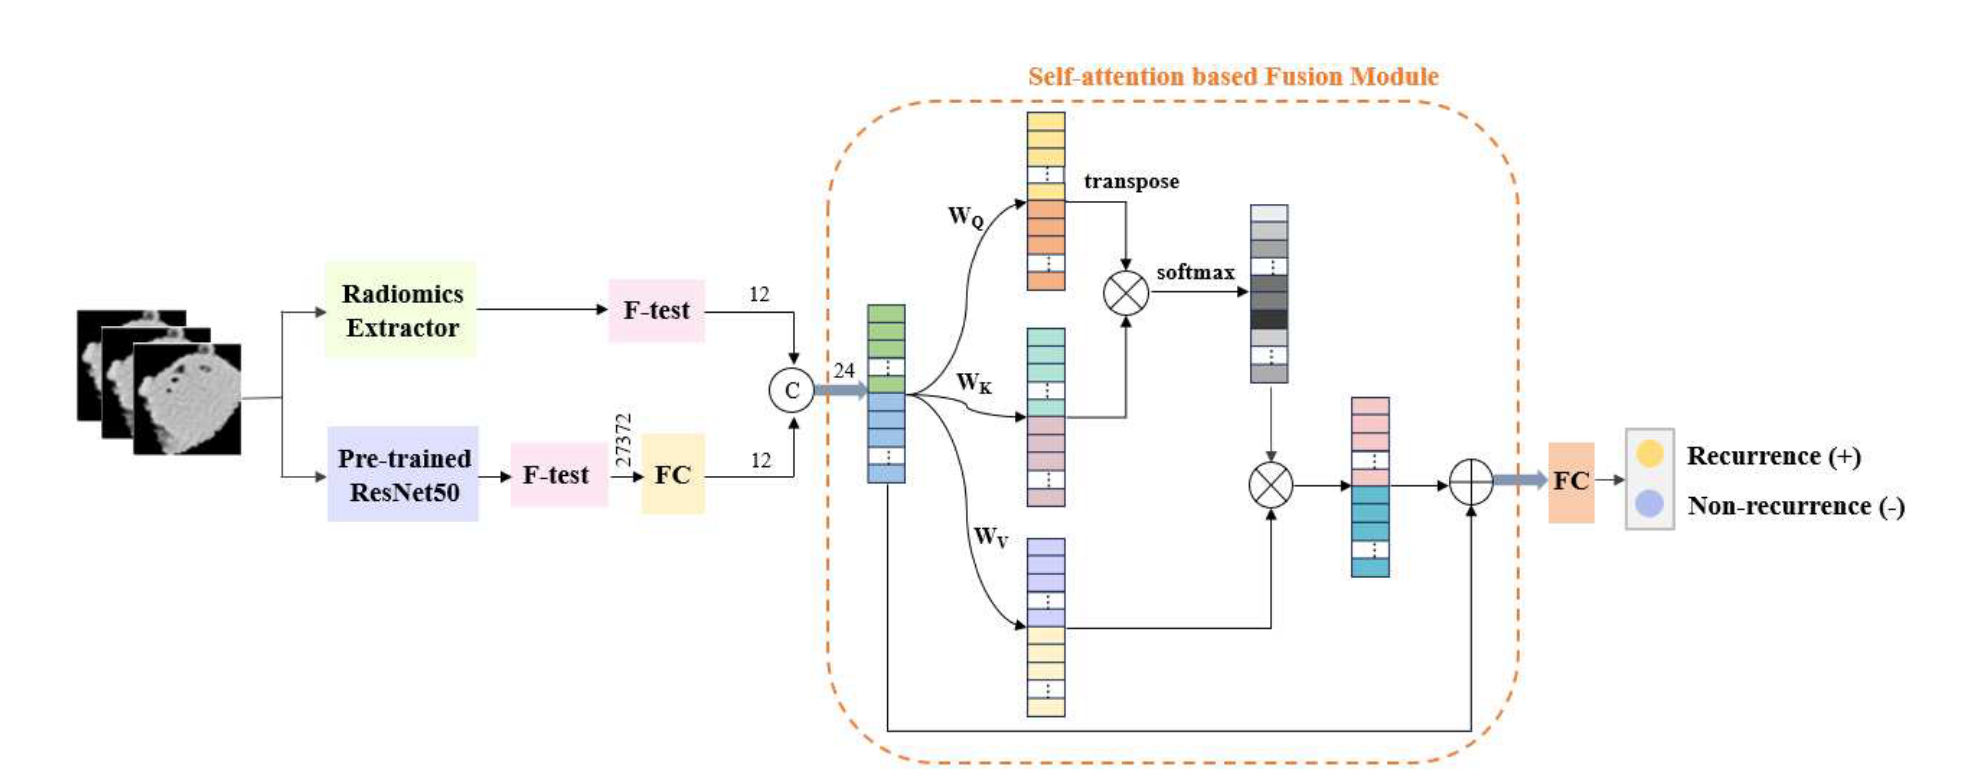
\includegraphics[width=\columnwidth]{figures/fig01.png}}
\caption{Proposed  Architecture for \gls{NSCLC} early recurrence prediction. First radiomic and deep features are extracrted, a F1-Test reduces their dimensions that are concatenated and sent ao a self-attention module.}
\label{fig01}
\end{figure}

% ------
\subsection{Proposed Model}

The schematic of the proposed architecture is shown in Figure \ref{fig02}. Deep features are extracted from the images and masks using ResNet50 and undergo a linear transformation to a size of $27,372$, as per the base model. Radiomic features are extracted by applying various statistical models, resulting in 78 features.

An F-Test set is applied to the feature vectors to ensure they have the same size, which is determined by the $\text{EMBED}_{size}$ parameter. The selected features are then concatenated and passed through the convolution module, which consists of a 1D convolution, an \gls{SE} block, and another 1D convolution. The first convolution converts the number of channels to $16$, the SE block maintains the dimensionality, and the second convolution reduces the channels from $16$ to $1$. The process continues through the self-attention module, and finally, a linear layer with a single neuron performs binary classification.


\begin{figure}[h]
\centerline{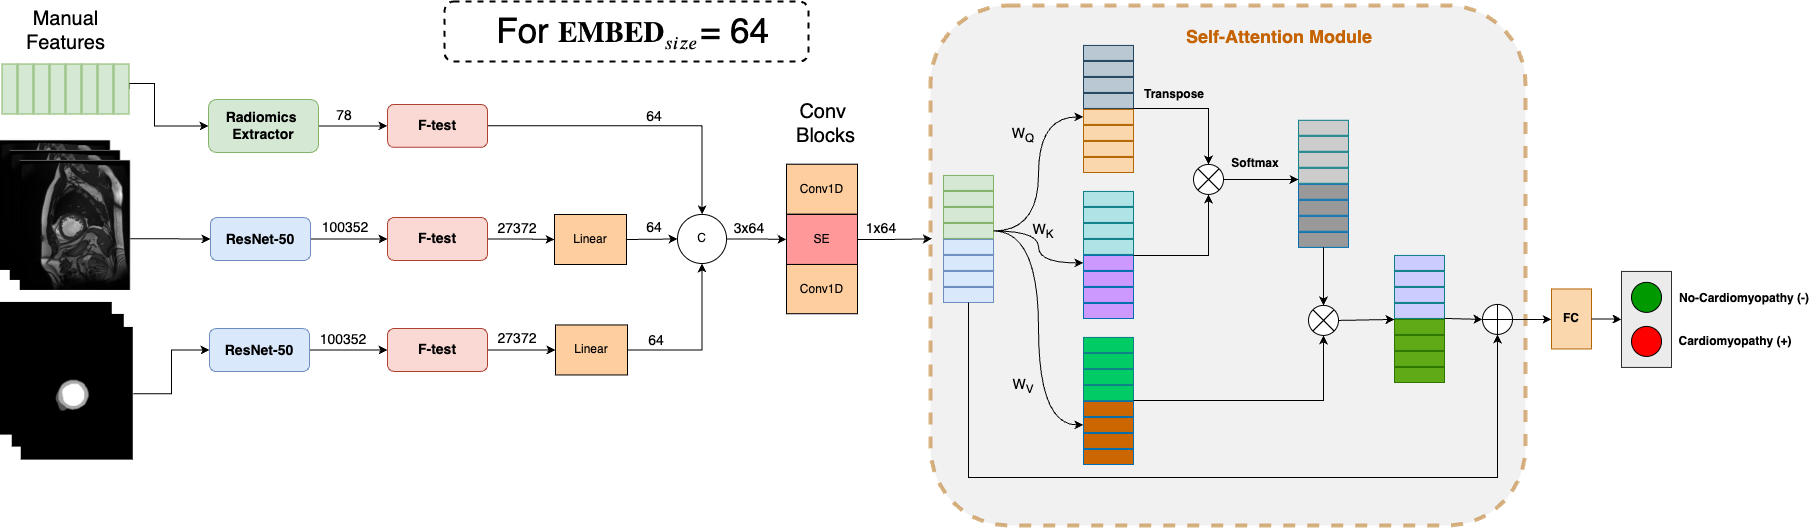
\includegraphics[width=\columnwidth]{figures/fig02.png}}
\caption{Proposed Architecture for cardiomyopathy classification. The concatenation are made in the channels dimension. There major difference are the addition of the heart mask, and the SE Module.}
\label{fig02}
\end{figure}

% ------
\subsection{Selective Attention Module}

Selective attention plays a crucial role in improving the performance of deep learning models by allowing them to focus on the most relevant features in their internal representations. Specifically, the \gls{SE} block is designed to adaptively recalibrate feature channels by assigning higher weights to the most informative characteristics. This mechanism operates in two main steps: first, it reduces the dimensionality of global features (squeeze) to capture overall context, and then it applies an excitation mechanism to adjust the weights of each channel based on their relative importance. By integrating \gls{SE} blocks into an architecture, the model enhances its ability to discriminate relevant patterns while suppressing noise or irrelevant information, leading to greater accuracy and efficiency in data processing \cite{yangNeuralNetworkDesign2024a}.

Since the \gls{SE} block is added only in the adapted version to improve results, the resulting concatenated vector is $3 \times 64$, assuming $\text{EMBED}_{size}= 64$ and the inclusion of the mask. A 1D convolutional layer is applied with $16$ channels, a kernel size of $3$, a stride of $1$, and padding of $1$ to maintain the original dimensions after processing \cite{huSqueezeandExcitationNetworks2018}.  

With $16$ channels as the output of the first convolution, the \gls{SE} block is applied to identify the most relevant channels and rescale the original input. The SE block has a reduction parameter $r$, which was set to $16$, as suggested by the authors of the original study. Finally, another 1D convolution is applied with a single output channel, resulting in a one-dimensional vector, which serves as input for the next block, the self-attention module.

% ------
\subsection{Self-Attention Module}

The self-attention mechanism was employed to learn the importance of each feature and capture long-range dependencies. As illustrated in Figure \ref{fig02}, the self-attention module is used to map a query ($Q$), key ($K$), and value ($V$) into an attention-weighted value.  

The model uses 24 concatenated features $F_{hd}$ in the original version and $\text{EMBED}_{size}$ features in the adapted versions. From the resulting vector, each feature is projected onto three learnable matrices: key matrix ($K$), query matrix ($Q$), and value matrix ($V$) through dot-product operations with their corresponding weight matrices $W_{Q}$, $W_{K}$, and $W_{V}$. Consequently, the values $Q$, $K$, and $V$ are defined as $W_{Q}F_{gd}$, $W_{K}F_{gd}$, and $W_{V}F_{gd}$, respectively, where $W_{Q}$, $W_{K}$, and $W_{V}$ represent the linear transformations applied to generate the matrices $Q$, $K$, and $V$ \cite{vaswaniAttentionAllYou2023}.  

The self-attention module is defined in Equation \ref{eq:attention}, where $d_{k}$ represents the dimension of $K$. Without requiring recurrent or convolutional operations, the self-attention module can model long-term dependencies between input features. This module adaptively computes feature weights based on their importance and relevance, enhancing the associations between radiomic and deep features \cite{vaswaniAttentionAllYou2023}.  

This process strengthens the expressive power of the fused features and enables the model to focus more precisely on the most informative features, assisting in medical image diagnosis while reducing the influence of irrelevant features in prediction. Additionally, the model can dynamically allocate attention to different cardiac MRI (\gls{MRI}) image samples, allowing for better adaptation to the feature representations of different cases, improving both accuracy and generalization.  

The loss function used in the model is the binary cross-entropy denoted by the Equation \ref{eq:bce}. Here, $\mathcal{L}_{bce}$ denotes \gls{BCE}, $N$ represents the number of cardiac \gls{MRI}, $r$ denotes the target class of cardiomyopathy, and $\hat{r}$ is the predicted value by the model. A value of 1 indicates the presence of cardiomyopathy, while 0 indicates its absence.

\begin{equation}
\text{Attention}(Q, K, V) = \text{softmax}\left(\frac{QK^T}{\sqrt{d_k}}\right)V
\label{eq:attention}
\end{equation}

\begin{equation}
\mathcal{L}_{bce} = -\frac{1}{N} \sum_{i=1}^N
(r_i \ln \hat{r}_i + (1 - r_i) \ln (1 - \hat{r}_i))
\label{eq:bce}
\end{equation}


% ---------------------------------------------
\section{Experiments and Results}

This chapter presents the results of the proof of concept conducted with the developed algorithms, including both the baseline model and the adapted models, with the goal of comparing them to the objectives outlined in this dissertation. The tests performed aim to evaluate the algorithm's efficiency under the various adaptations discussed.

% ------
\subsection{Experiments Base Model}

A proof of concept was conducted on the ACDC dataset using the baseline model for an initial evaluation, which was also used as the baseline reference. The baseline model was implemented according to the original paper, and its implementation is shown in Figure \ref{fig01}.  

The training dataset consists of $100$ patient exams, considering only image slices from the diastolic phase. First-order features were extracted using the \textit{PyRadiomics} library, resulting in 78 values that compose the radiomic features.  

For deep feature extraction, a frozen ResNet50 network was used, excluding its final linear layer, which was originally responsible for classifying $1,000$ classes from the ImageNet dataset. The final output was a feature vector containing $100,352$ deep features.  

In this experiment, the model was trained using binary cross-entropy as the objective function, a learning rate of 0.0001, the Adam optimizer, a batch size of 1, and approximately 60 epochs. During training, it was observed that the error stabilized over time. Additionally, a data randomization strategy was employed during training. Finally, the sigmoid function was applied to the output vector of the model so we a probability result between $0$ and $1$. For the classification, it was considered that values above $0,5$ are considered cardiomyopathy and value below or equal $0,5$ are considered normal cases.

% ------
\subsection{Experiments Adapted Model}

The adapted models represent modifications derived from the baseline model, aiming to evaluate whether changes either in hyperparameters or in architectural components can yield promising improvements over the baseline results. These modifications can be categorized as follows:  

\begin{enumerate}  

\item Changes to $\text{EMBED}_{size}$, where the values $[24, 48, 64]$ were tested in an attempt to preserve more of the original information.  

\item In the adapted versions, the respective masks are also incorporated and later concatenated with the radiomic and deep features.  

\item The concatenation process differs from the original model. For instance, assuming $\text{EMBED}_{size} = 12$, the original version produces a $1\times24$ output, whereas in the adapted version, concatenation is performed along the first dimension, resulting in a $2\times12$ output. This adjustment is made because the adapted model introduces a new convolutional block, consisting of a convolution operation and \gls{SE} blocks.  

\end{enumerate}  

The remaining architecture follows the original design, except that the self-attention block can be applied $N$ times. This means its output is recursively fed back as input $N$ times, making $N$ a tunable hyperparameter in the experiment. The tested values for $N$ were $[1, 2, 4, 6]$. These changes do not alter the overall structure of the initial architecture but allow the self-attention module to be executed $N$ times, as proposed in \cite{vaswaniAttentionAllYou2023} and seen in Figure \ref{fig03}.

\begin{figure}[h]
\centerline{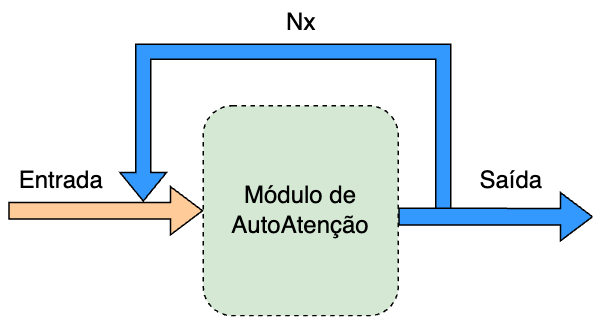
\includegraphics[width=\columnwidth]{figures/fig03.png}}
\caption{Self-attention module recurrence.}
\label{fig03}
\end{figure}

% ------
\subsection{Results Base Model}

With the preprocessed and previously stored data, training is performed using the radiomic and deep feature vectors. Partial metrics were saved in real time during training.  For the baseline model, the hyperparameters are: $\text{EMBED}_{size} = 12$, $N = 1$ (i.e., a single self-attention block), concatenation dimension = 1, learning rate = $0,0001$, optimizer Adam, batch size = $1$ and approximately $60$ epochs.

Once trained, inference was performed on the test dataset, applying the sigmoid function and setting 0.5 as the decision threshold, where values above this threshold are classified as cardiomyopathy, while the others are classified as normal.  

The resulting metrics can be found in Table \ref{tab:metrics}. The confusion matrix is shown in Figure \ref{fig05}.
% , and a graph illustrating the ROC curve is presented in Figure \ref{fig:fig017}.

\begin{table}[h!]
    \centering
    \caption{Experiment Metrica - Base Model}
    \begin{tabular}{|c|c|}
    \hline 
          \textbf{Metric} & \textbf{Value} \\ 
    \hline 
        Accuracy & 0.58 \\ 
    \hline 
        Precision & 0.47 \\ 
    \hline 
        Recall & 0.45 \\ 
    \hline 
        AUC & 0.55 \\ 
    \hline 
    \end{tabular} 
    \label{tab:metrics}
\end{table}

\begin{figure}[h]
    \centerline{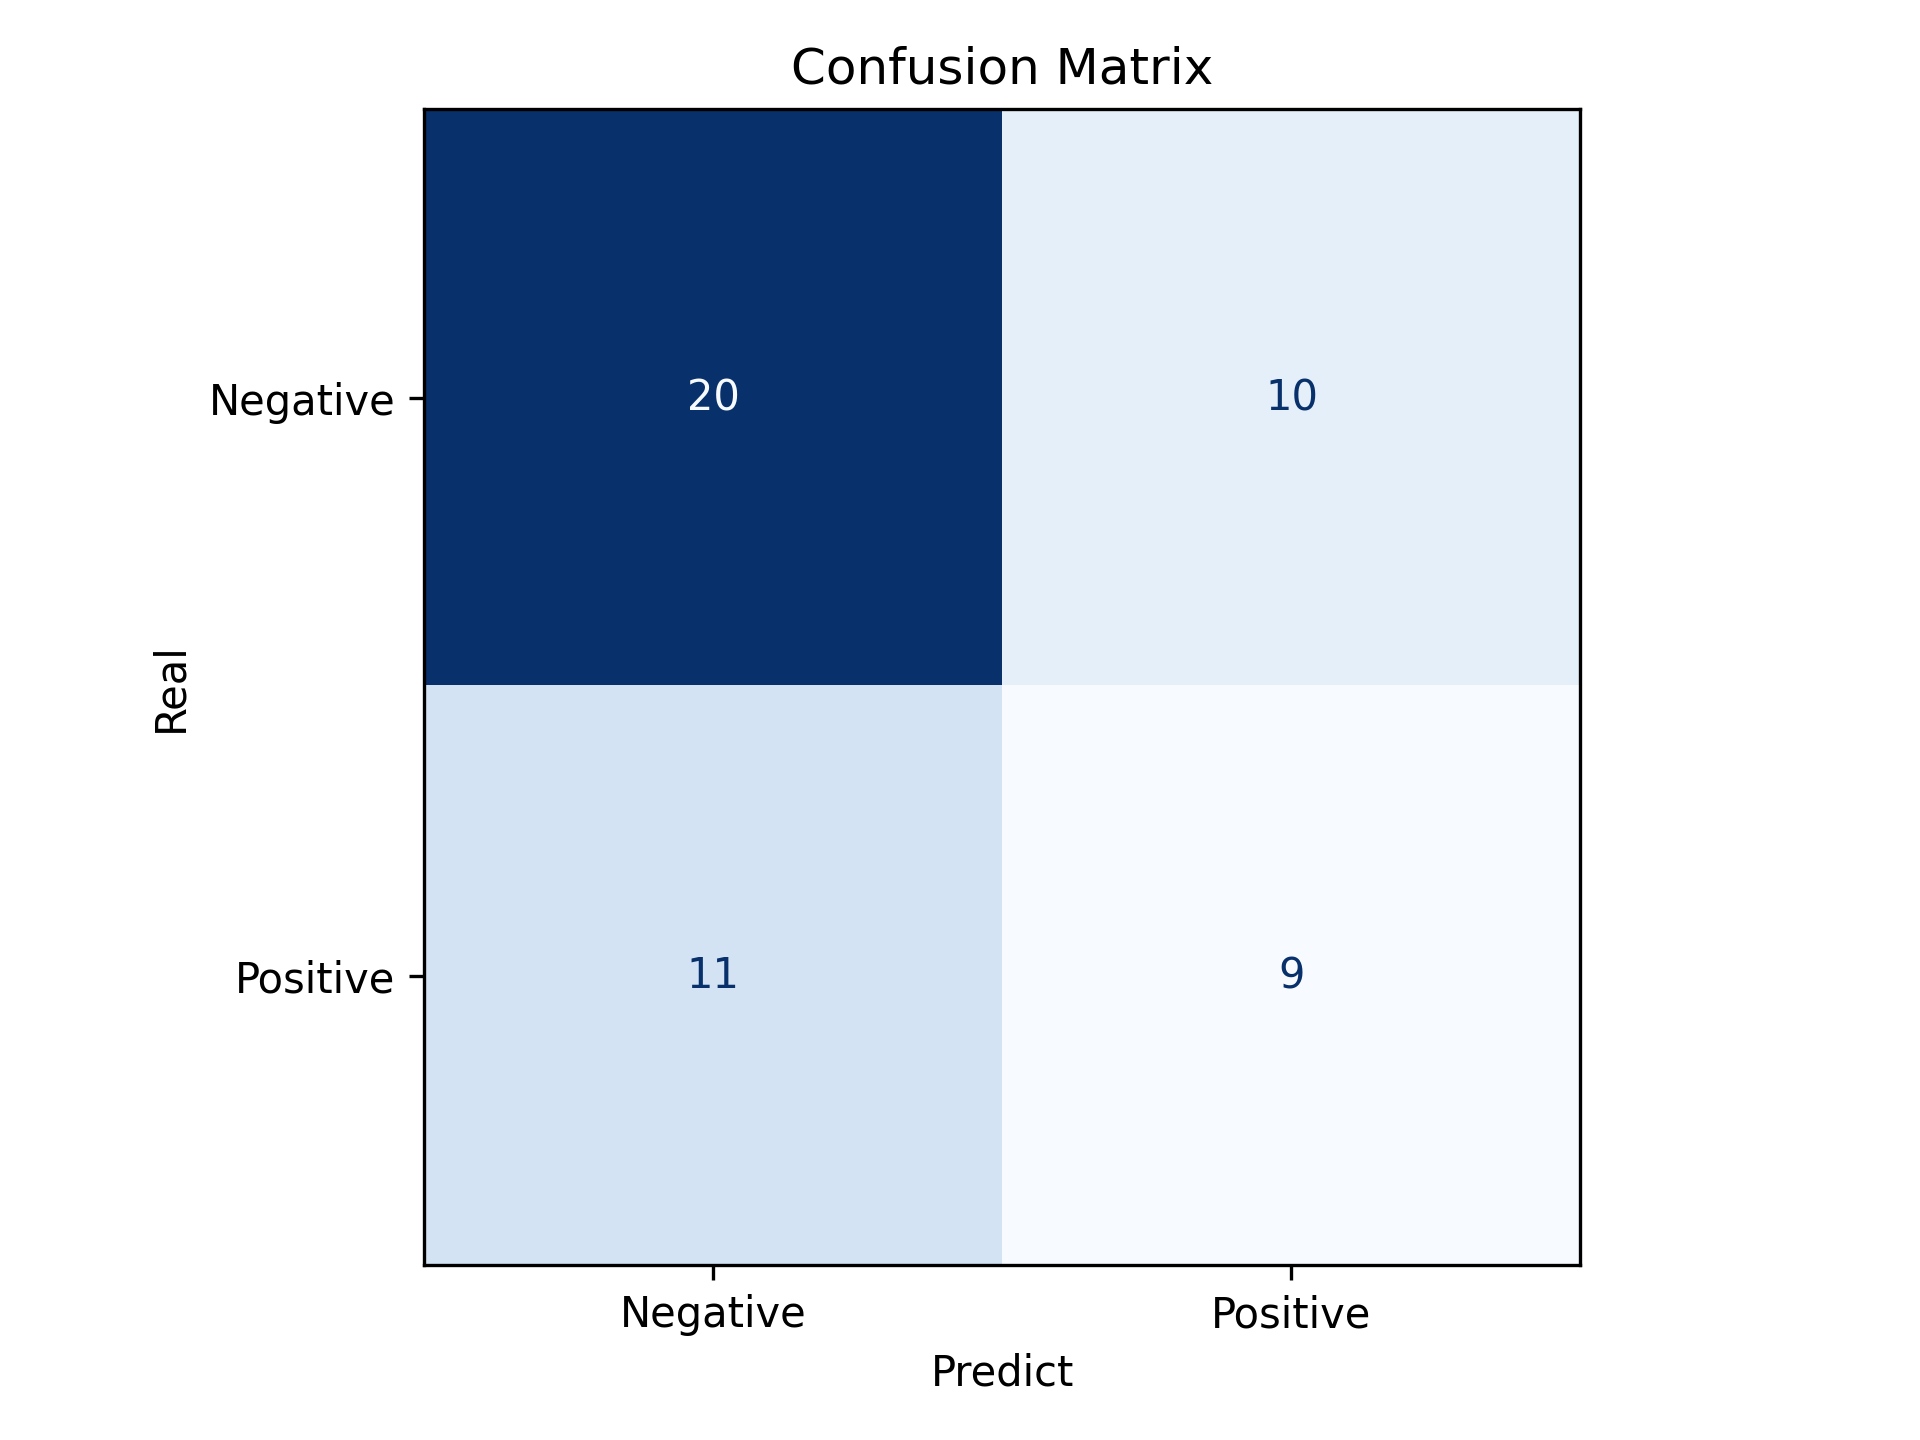
\includegraphics[width=\columnwidth]{figures/fig05.png}}
    \caption{Confusion Matrix -  Base Model.}
    \label{fig05}
\end{figure}


% ------
\subsection{Results Adapted Model}

For the adapted versions, the objective was to modify both the hyperparameters and the model architecture to compare the results with the baseline version. The first experiments were conducted by varying the $\text{EMBED}_{size}$, and the self-attention block was applied $N$ times instead of just once. These experiments were executed by generating combinations of these hyperparameters to cover as many scenarios as possible within the proposed methodology.  

Additionally, a convolutional module was introduced in the adapted versions, preceding the self-attention module. This convolutional module consists of three blocks: a 1D convolutional layer, an \gls{SE} block, and another 1D convolutional block. With the option to add a third feature vector, represented by the mask, it became possible to identify intrinsic relationships involving this additional vector. The concatenation is now performed along the first dimension, making each feature vector a separate channel.  

In the convolutional module, the first 1D convolutional layer increases the number of channels to 16, meaning that 16 filters are applied for spatial information extraction. The \gls{SE} block represents the selective attention layer, which assigns importance to the most relevant channels by identifying their significance and scaling them in the original input using an optimized scalar value learned during training. Further details can be seen in Figure \ref{fig06}. In this project, the \gls{SE} block is adapted for 1D applications, unlike the original study, which focuses on its use in well-established computer vision models. The reduction factor $r$ in the \gls{SE} block was fixed at 16, as empirical tests conducted by the original study's authors confirmed that this value yields the best results.


\begin{figure}[h]
    \centerline{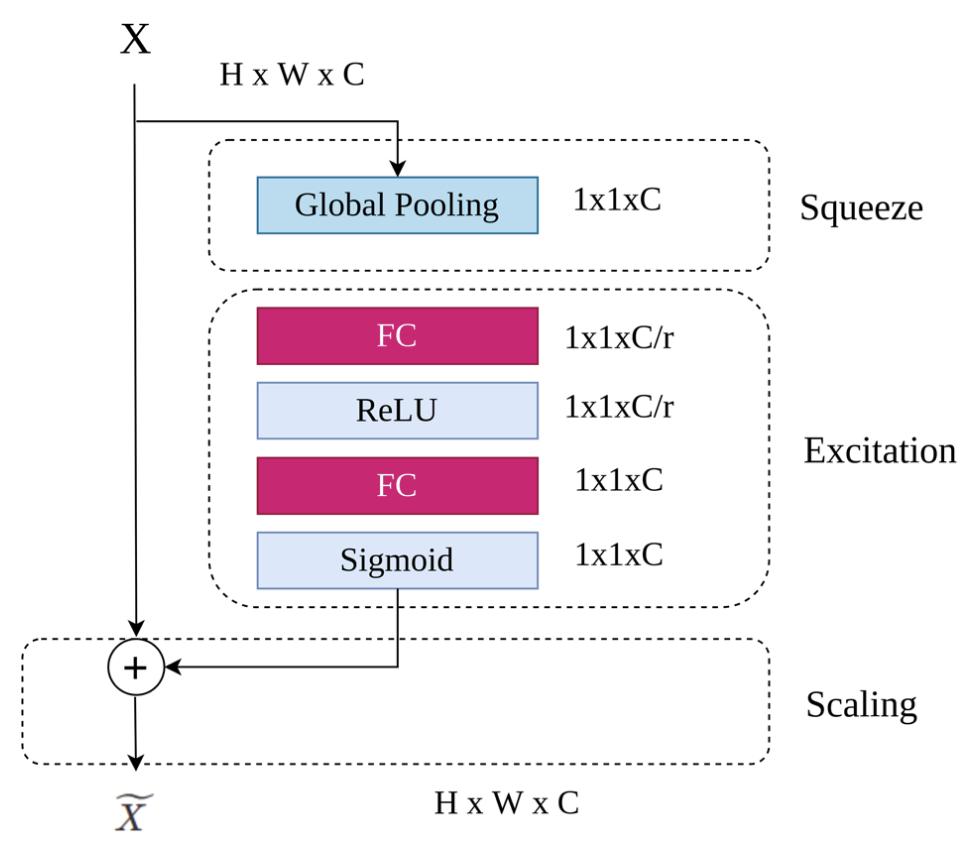
\includegraphics[width=\columnwidth]{figures/fig06.png}}
    \caption{SE Block Composition}
    \label{fig06}
\end{figure}

As we already have the base models results,  Table \ref{tab:metrics_acdc_orig_mask} shows the experiments that include the mask as a third feature vector and Table \ref{tab:metrics_acdc_se} presents the addition of convolutional and \gls{SE} blocks.  

Several observations can be made from the experiment. The training process almost always exhibits overfitting, reaching nearly $100$\% accuracy. This can be justified by the limited number of training samples available. Another notable point is that larger feature vector sizes (Emb) tend to yield better results. Additionally, increasing the number of self-attention blocks (N\_Attn) also improves performance, except when set to 6. This is likely due to the model becoming overly complex compared to the available training data, negatively impacting its generalization ability.  

The best results were obtained in versions that incorporated the \gls{SE} block and used four self-attention blocks, with the best experiment achieving $78$\% accuracy.


\begin{table}[htbp]
\centering
\caption{ACDC Metrics - Adapted Models + Masks
\newline Bold means better Acc.}
\begin{tabular}{lcccccc}
\toprule
\textbf{Emb} & \textbf{N\_Attn} & \textbf{Acc} & \textbf{Precision} & \textbf{Recall} & \textbf{F1} & \textbf{AUC} \\
\midrule
24 & 1 & 0.44 & 0.35 & 0.45 & 0.39 & 0.44 \\
24 & 2 & 0.46 & 0.38 & 0.55 & 0.45 & 0.48 \\
24 & 4 & 0.48 & 0.36 & 0.40 & 0.38 & 0.47 \\
24 & 6 & 0.48 & 0.38 & 0.45 & 0.41 & 0.47 \\
\hline
48 & 1 & 0.52 & 0.44 & 0.70 & 0.54 & 0.55 \\
48 & 2 & 0.58 & 0.48 & 0.55 & 0.51 & 0.57 \\
48 & 4 & 0.62 & 0.52 & 0.60 & 0.56 & 0.62 \\
48 & 6 & 0.60 & 0.50 & 0.50 & 0.50 & 0.58 \\
\hline
64 & 1 & 0.58 & 0.48 & 0.60 & 0.53 & 0.58 \\
64 & 2 & 0.56 & 0.45 & 0.50 & 0.48 & 0.55 \\
\textbf{64} & \textbf{4} & \textbf{0.64} & \textbf{0.54} & \textbf{0.65} & \textbf{0.59} & \textbf{0.64} \\
64 & 6 & 0.62 & 0.53 & 0.45 & 0.49 & 0.59 \\
\bottomrule
\end{tabular}
\label{tab:metrics_acdc_orig_mask}
\end{table}


\begin{table}[htbp]
\centering
\caption{ACDC Metrics - Adapted Models + Masks + SE Blocks 
\newline Bold means better Acc.}
\begin{tabular}{lcccccc}
\toprule
\textbf{Emb} & \textbf{N\_Attn} & \textbf{Acc} & \textbf{Precision} & \textbf{Recall} & \textbf{F1} & \textbf{AUC} \\
\midrule
24 & 1 & 0.66 & 0.56 & 0.70 & 0.62 & 0.67 \\
24 & 2 & 0.68 & 0.58 & 0.75 & 0.65 & 0.69 \\
24 & 4 & 0.70 & 0.59 & 0.80 & 0.68 & 0.72 \\
24 & 6 & 0.68 & 0.59 & 0.65 & 0.62 & 0.67 \\
\hline
48 & 1 & 0.70 & 0.58 & 0.90 & 0.71 & 0.73 \\
48 & 2 & 0.70 & 0.62 & 0.65 & 0.63 & 0.69 \\
48 & 4 & 0.74 & 0.65 & 0.75 & 0.70 & 0.74 \\
48 & 6 & 0.70 & 0.60 & 0.75 & 0.67 & 0.71 \\
\hline
64 & 1 & 0.64 & 0.54 & 0.65 & 0.59 & 0.64 \\
64 & 2 & 0.72 & 0.64 & 0.70 & 0.67 & 0.72 \\
\textbf{64} & \textbf{4} & \textbf{0.78} & \textbf{0.76} & \textbf{0.65} & \textbf{0.70} & \textbf{0.76} \\
64 & 6 & 0.76 & 0.65 & 0.85 & 0.74 & 0.77 \\
\bottomrule
\end{tabular}
\label{tab:metrics_acdc_se}
\end{table}








% ---------------------------------------------
\section{Conclusion}

This study presented an innovative approach for the classification of cardiomyopathies using cardiac \gls{MRI} images combined with attention mechanisms, promoting the integration of radiomic and deep features. The proposed method was built on strong theoretical foundations, employing modern deep learning techniques, such as the \gls{SE} Net architecture and self-attention mechanisms, to explore discriminative features in medical images.  

The results highlighted the efficiency of the proposed model in identifying patterns associated with cardiomyopathies, surpassing traditional approaches in terms of accuracy and generalization. The fusion of radiomic information, which captures textural and statistical details, with deep features extracted from convolutional networks, proved to be effective in handling the intrinsic complexity of cardiomyopathies. Additionally, the use of attention mechanisms allowed the model to prioritize the most relevant regions of the images, enhancing its expressiveness.  

The use of SE and spatial attention in the medical imaging domain represented an innovative strategy by prioritizing relevant information in the feature map. This technique not only improved the model’s performance but also provided a more intuitive way to explain AI decisions, a crucial aspect for its acceptance in clinical practice.  

Although the results are promising, this study also revealed limitations, such as the need for more robust and diverse datasets and the challenge of interpreting deep learning models, a recurring issue in medical AI applications. 

% However, the proposed model represents a significant advancement in the application of artificial intelligence to medical diagnostics, contributing to the development of more precise and accessible tools for clinical decision support, especially for early diagnosis and monitoring of cardiomyopathies. These tools can enhance healthcare efficiency, reduce manual analysis time, and enable faster, more precise interventions.  

For future work, it is suggested to explore the combination of medical images with clinical and genetic data to create multimodal models capable of providing more holistic and personalized diagnoses. 


% ---------------------------------------------
\appendices

\section*{Acknowledgment}

\lipsum[11-11]


\section*{References and Footnotes}
\subsection{References}
% \begin{thebibliography}{00}

\bibitem{b1} G. O. Young, ``Synthetic structure of industrial plastics,'' in \emph{Plastics,} 2\textsuperscript{nd} ed., vol. 3, J. Peters, Ed. New York, NY, USA: McGraw-Hill, 1964, pp. 15--64.

\bibitem{b2} W.-K. Chen, \emph{Linear Networks and Systems.} Belmont, CA, USA: Wadsworth, 1993, pp. 123--135.

\bibitem{b3} J. U. Duncombe, ``Infrared navigation---Part I: An assessment of feasibility,'' \emph{IEEE Trans. Electron Devices}, vol. ED-11, no. 1, pp. 34--39, Jan. 1959, 10.1109/TED.2016.2628402.

\bibitem{b4} E. P. Wigner, ``Theory of traveling-wave optical laser,'' \emph{Phys. Rev}., vol. 134, pp. A635--A646, Dec. 1965.

\bibitem{b5} E. H. Miller, ``A note on reflector arrays,'' \emph{IEEE Trans. Antennas Propagat}., to be published.

\bibitem{b6} E. E. Reber, R. L. Michell, and C. J. Carter, ``Oxygen absorption in the earth's atmosphere,'' Aerospace Corp., Los Angeles, CA, USA, Tech. Rep. TR-0200 (4230-46)-3, Nov. 1988.

\bibitem{b7} J. H. Davis and J. R. Cogdell, ``Calibration program for the 16-foot antenna,'' Elect. Eng. Res. Lab., Univ. Texas, Austin, TX, USA, Tech. Memo. NGL-006-69-3, Nov. 15, 1987.

\bibitem{b8} \emph{Transmission Systems for Communications}, 3\textsuperscript{rd} ed., Western Electric Co., Winston-Salem, NC, USA, 1985, pp. 44--60.

\bibitem{b9} \emph{Motorola Semiconductor Data Manual}, Motorola Semiconductor Products Inc., Phoenix, AZ, USA, 1989.

\bibitem{b10} G. O. Young, ``Synthetic structure of industrial
plastics,'' in Plastics, vol. 3, Polymers of Hexadromicon, J. Peters,
Ed., 2\textsuperscript{nd} ed. New York, NY, USA: McGraw-Hill, 1964, pp. 15-64.
[Online]. Available:
\underline{http://www.bookref.com}.

\bibitem{b11} \emph{The Founders' Constitution}, Philip B. Kurland
and Ralph Lerner, eds., Chicago, IL, USA: Univ. Chicago Press, 1987.
[Online]. Available: \underline{http://press-pubs.uchicago.edu/founders/}

\bibitem{b12} The Terahertz Wave eBook. ZOmega Terahertz Corp., 2014.
[Online]. Available:
\underline{http://dl.z-thz.com/eBook/zomega\_ebook\_pdf\_1206\_sr.pdf}. Accessed on: May 19, 2014.

\bibitem{b13} Philip B. Kurland and Ralph Lerner, eds., \emph{The
Founders' Constitution.} Chicago, IL, USA: Univ. of Chicago Press,
1987, Accessed on: Feb. 28, 2010, [Online] Available:
\underline{http://press-pubs.uchicago.edu/founders/}

\bibitem{b14} J. S. Turner, ``New directions in communications,'' \emph{IEEE J. Sel. Areas Commun}., vol. 13, no. 1, pp. 11-23, Jan. 1995.

\bibitem{b15} W. P. Risk, G. S. Kino, and H. J. Shaw, ``Fiber-optic frequency shifter using a surface acoustic wave incident at an oblique angle,'' \emph{Opt. Lett.}, vol. 11, no. 2, pp. 115--117, Feb. 1986.

\bibitem{b16} P. Kopyt \emph{et al., ``}Electric properties of graphene-based conductive layers from DC up to terahertz range,'' \emph{IEEE THz Sci. Technol.,} to be published. DOI: 10.1109/TTHZ.2016.2544142.

\bibitem{b17} PROCESS Corporation, Boston, MA, USA. Intranets:
Internet technologies deployed behind the firewall for corporate
productivity. Presented at INET96 Annual Meeting. [Online].
Available: \underline{http://home.process.com/Intranets/wp2.htp}

\bibitem{b18} R. J. Hijmans and J. van Etten, ``Raster: Geographic analysis and modeling with raster data,'' R Package Version 2.0-12, Jan. 12, 2012. [Online]. Available: \underline {http://CRAN.R-project.org/package=raster} 

\bibitem{b19} Teralyzer. Lytera UG, Kirchhain, Germany [Online].
Available:
\underline{http://www.lytera.de/Terahertz\_THz\_Spectroscopy.php?id=home}, Accessed on: Jun. 5, 2014

\bibitem{b20} U.S. House. 102\textsuperscript{nd} Congress, 1\textsuperscript{st} Session. (1991, Jan. 11). \emph{H. Con. Res. 1, Sense of the Congress on Approval of}  \emph{Military Action}. [Online]. Available: LEXIS Library: GENFED File: BILLS

\bibitem{b21} Musical toothbrush with mirror, by L.M.R. Brooks. (1992, May 19). Patent D 326 189 [Online]. Available: NEXIS Library: LEXPAT File: DES

\bibitem{b22} D. B. Payne and J. R. Stern, ``Wavelength-switched pas- sively coupled single-mode optical network,'' in \emph{Proc. IOOC-ECOC,} Boston, MA, USA, 1985, pp. 585--590.

\bibitem{b23} D. Ebehard and E. Voges, ``Digital single sideband detection for interferometric sensors,'' presented at the \emph{2\textsuperscript{nd} Int. Conf. Optical Fiber Sensors,} Stuttgart, Germany, Jan. 2-5, 1984.

\bibitem{b24} G. Brandli and M. Dick, ``Alternating current fed power supply,'' U.S. Patent 4 084 217, Nov. 4, 1978.

\bibitem{b25} J. O. Williams, ``Narrow-band analyzer,'' Ph.D. dissertation, Dept. Elect. Eng., Harvard Univ., Cambridge, MA, USA, 1993.

\bibitem{b26} N. Kawasaki, ``Parametric study of thermal and chemical nonequilibrium nozzle flow,'' M.S. thesis, Dept. Electron. Eng., Osaka Univ., Osaka, Japan, 1993.

\bibitem{b27} A. Harrison, private communication, May 1995.

\bibitem{b28} B. Smith, ``An approach to graphs of linear forms,'' unpublished.

\bibitem{b29} A. Brahms, ``Representation error for real numbers in binary computer arithmetic,'' IEEE Computer Group Repository, Paper R-67-85.

\bibitem{b30} IEEE Criteria for Class IE Electric Systems, IEEE Standard 308, 1969.

\bibitem{b31} Letter Symbols for Quantities, ANSI Standard Y10.5-1968.

\bibitem{b32} R. Fardel, M. Nagel, F. Nuesch, T. Lippert, and A. Wokaun, ``Fabrication of organic light emitting diode pixels by laser-assisted forward transfer,'' \emph{Appl. Phys. Lett.}, vol. 91, no. 6, Aug. 2007, Art. no. 061103.~

\bibitem{b33} J. Zhang and N. Tansu, ``Optical gain and laser characteristics of InGaN quantum wells on ternary InGaN substrates,'' \emph{IEEE Photon. J.}, vol. 5, no. 2, Apr. 2013, Art. no. 2600111

\bibitem{b34} S. Azodolmolky~\emph{et al.}, Experimental demonstration of an impairment aware network planning and operation tool for transparent/translucent optical networks,''~\emph{J. Lightw. Technol.}, vol. 29, no. 4, pp. 439--448, Sep. 2011.

\end{thebibliography}

% \bibliographystyle{IEEEtranN}
\bibliographystyle{plain}
\bibliography{refs}

\end{document}
